% Figure per il Capitolo 4 - Codice TikZ
% Da inserire nel preambolo del documento principale:
\usepackage{tikz}
\usepackage{pgfplots}
\usetikzlibrary{shapes,arrows,positioning,calc,patterns,decorations.pathreplacing,shadows,fit}
\pgfplotsset{compat=1.17}
\begin{document}


% =================================================================
% FIGURA 4.1: Diagramma di Venn - Sovrapposizioni Normative
% =================================================================
\begin{figure}[h]
\centering
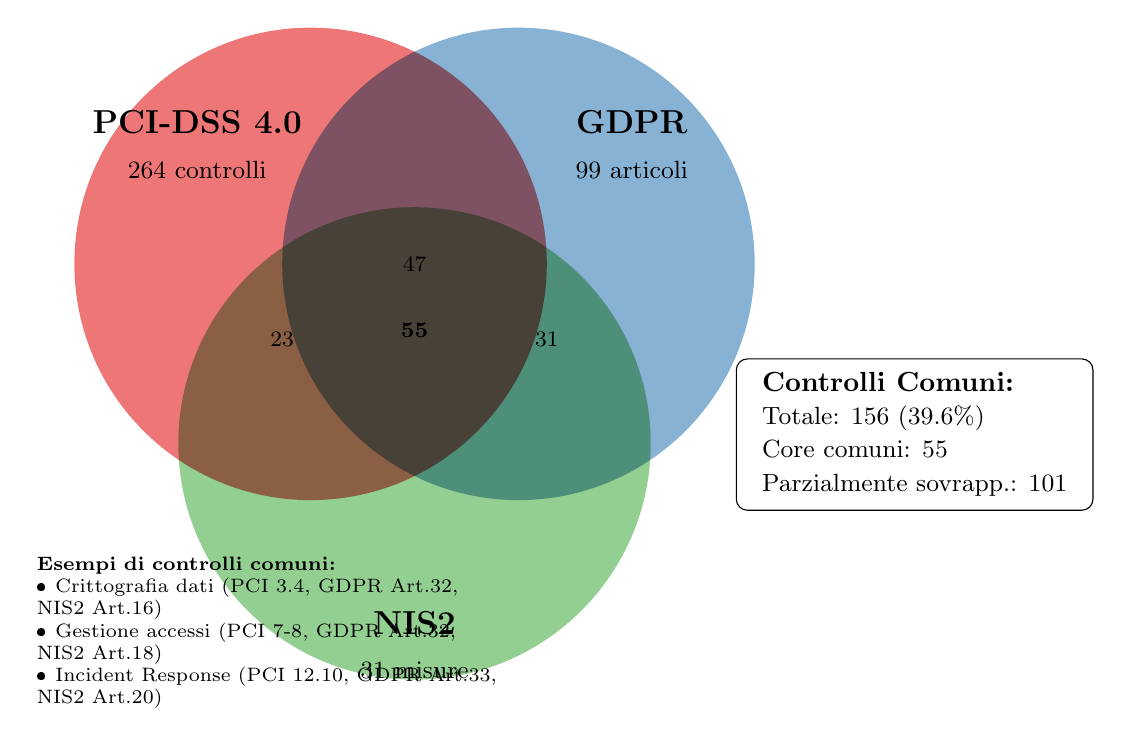
\begin{tikzpicture}[scale=1.2]
    % Definizione colori
    \definecolor{pcidss}{RGB}{228,26,28}
    \definecolor{gdpr}{RGB}{55,126,184}
    \definecolor{nis2}{RGB}{77,175,74}
    
    % Cerchi principali con trasparenza
    \begin{scope}[blend mode=multiply]
        % PCI-DSS
        \fill[pcidss,opacity=0.6] (0,0) circle (2.5cm);
        % GDPR
        \fill[gdpr,opacity=0.6] (2.2,0) circle (2.5cm);
        % NIS2
        \fill[nis2,opacity=0.6] (1.1,-1.9) circle (2.5cm);
    \end{scope}
    
    % Etichette dei cerchi
    \node[font=\bfseries\large] at (-1.2,1.5) {PCI-DSS 4.0};
    \node[font=\small] at (-1.2,1) {264 controlli};
    
    \node[font=\bfseries\large] at (3.4,1.5) {GDPR};
    \node[font=\small] at (3.4,1) {99 articoli};
    
    \node[font=\bfseries\large] at (1.1,-3.8) {NIS2};
    \node[font=\small] at (1.1,-4.3) {31 misure};
    
    % Annotazioni delle intersezioni
    \node[font=\footnotesize] at (1.1,0) {47};
    \node[font=\footnotesize] at (-0.3,-0.8) {23};
    \node[font=\footnotesize] at (2.5,-0.8) {31};
    \node[font=\footnotesize\bfseries] at (1.1,-0.7) {55};
    
    % Legenda delle sovrapposizioni
    \node[anchor=north west, draw, fill=white, rounded corners] at (4.5,-1) {
        \begin{tabular}{l}
        \textbf{Controlli Comuni:} \\
        \small Totale: 156 (39.6\%) \\
        \small Core comuni: 55 \\
        \small Parzialmente sovrapp.: 101
        \end{tabular}
    };
    
    % Esempi di controlli comuni
    \node[anchor=north west, text width=6cm, font=\scriptsize] at (-3,-3) {
        \textbf{Esempi di controlli comuni:}\\
        • Crittografia dati (PCI 3.4, GDPR Art.32, NIS2 Art.16)\\
        • Gestione accessi (PCI 7-8, GDPR Art.32, NIS2 Art.18)\\
        • Incident Response (PCI 12.10, GDPR Art.33, NIS2 Art.20)
    };
\end{tikzpicture}
\caption{Sovrapposizioni tra i principali standard normativi nel settore retail}
\label{fig:normative_overlap}
\end{figure}

% =================================================================
% FIGURA 4.2: Architettura a Tre Livelli
% =================================================================
\begin{figure}[h]
\centering
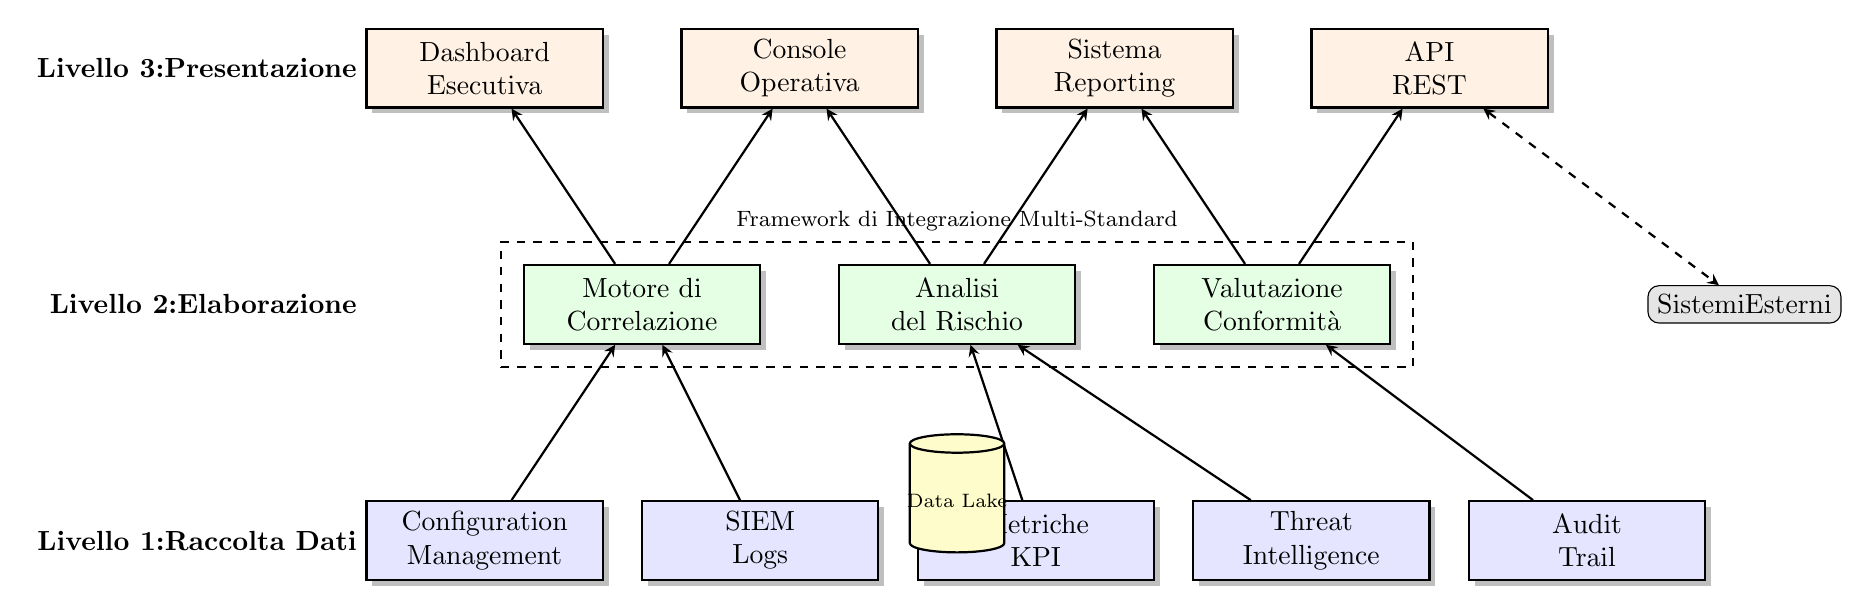
\begin{tikzpicture}[
    box/.style={rectangle, draw, thick, fill=white, drop shadow, minimum width=3cm, minimum height=1cm, align=center},
    databox/.style={box, fill=blue!10},
    processbox/.style={box, fill=green!10},
    presentbox/.style={box, fill=orange!10},
    arrow/.style={->, >=stealth, thick},
    doublearrow/.style={<->, >=stealth, thick}
]
    % Livello 3 - Presentazione
    \node[presentbox] (dashboard) at (0,6) {Dashboard\\Esecutiva};
    \node[presentbox] (console) at (4,6) {Console\\Operativa};
    \node[presentbox] (report) at (8,6) {Sistema\\Reporting};
    \node[presentbox] (api) at (12,6) {API\\REST};
    
    % Etichetta Livello 3
    \node[anchor=east, font=\bfseries] at (-1.5,6) {Livello 3:\\Presentazione};
    
    % Livello 2 - Analisi e Correlazione
    \node[processbox] (correlation) at (2,3) {Motore di\\Correlazione};
    \node[processbox] (risk) at (6,3) {Analisi\\del Rischio};
    \node[processbox] (compliance) at (10,3) {Valutazione\\Conformità};
    
    % Etichetta Livello 2
    \node[anchor=east, font=\bfseries] at (-1.5,3) {Livello 2:\\Elaborazione};
    
    % Livello 1 - Raccolta Dati
    \node[databox] (config) at (0,0) {Configuration\\Management};
    \node[databox] (siem) at (3.5,0) {SIEM\\Logs};
    \node[databox] (metrics) at (7,0) {Metriche\\KPI};
    \node[databox] (threat) at (10.5,0) {Threat\\Intelligence};
    \node[databox] (audit) at (14,0) {Audit\\Trail};
    
    % Etichetta Livello 1
    \node[anchor=east, font=\bfseries] at (-1.5,0) {Livello 1:\\Raccolta Dati};
    
    % Frecce tra livelli
    \draw[arrow] (config) -- (correlation);
    \draw[arrow] (siem) -- (correlation);
    \draw[arrow] (metrics) -- (risk);
    \draw[arrow] (threat) -- (risk);
    \draw[arrow] (audit) -- (compliance);
    
    \draw[arrow] (correlation) -- (dashboard);
    \draw[arrow] (correlation) -- (console);
    \draw[arrow] (risk) -- (console);
    \draw[arrow] (risk) -- (report);
    \draw[arrow] (compliance) -- (report);
    \draw[arrow] (compliance) -- (api);
    
    % Box di integrazione
    \node[draw, dashed, thick, fit=(correlation) (risk) (compliance), inner sep=8pt, label={[font=\footnotesize]above:Framework di Integrazione Multi-Standard}] {};
    
    % Sistemi esterni
    \node[draw, rounded corners, fill=gray!20] (external) at (16,3) {Sistemi\\Esterni};
    \draw[doublearrow, dashed] (api) -- (external);
    
    % Database centrale
    \node[cylinder, draw, thick, fill=yellow!20, shape border rotate=90, minimum height=1.5cm, minimum width=1.2cm] (db) at (6,0.5) {};
    \node[font=\scriptsize] at (6,0.5) {Data Lake};
\end{tikzpicture}
\caption{Architettura del sistema di conformità integrata}
\label{fig:architettura_sistema}
\end{figure}

% =================================================================
% FIGURA 4.3: Flusso di Processo GDPR
% =================================================================
\begin{figure}[h]
\centering
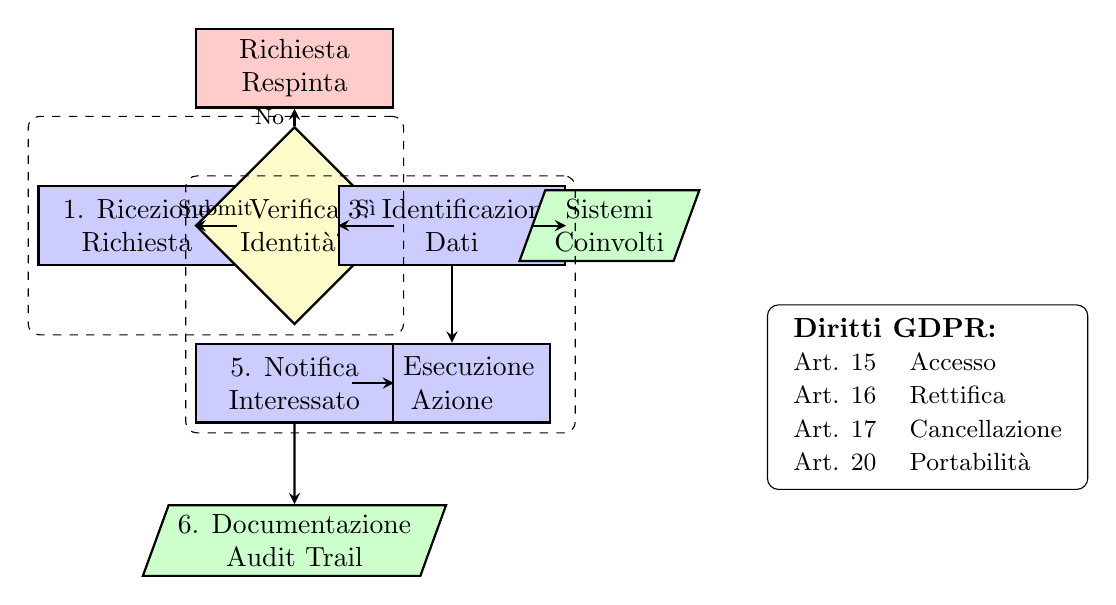
\begin{tikzpicture}[
    node distance=2cm,
    process/.style={rectangle, draw, thick, fill=blue!20, minimum width=2.5cm, minimum height=1cm, align=center},
    decision/.style={diamond, draw, thick, fill=yellow!20, minimum width=2cm, minimum height=1cm, align=center},
    data/.style={trapezium, trapezium left angle=70, trapezium right angle=110, draw, thick, fill=green!20, minimum width=2cm, minimum height=0.8cm, align=center},
    arrow/.style={->, >=stealth, thick},
    label/.style={font=\footnotesize}
]
    % Nodi del processo
    \node[process] (receive) {1. Ricezione\\Richiesta};
    \node[decision, right of=receive] (verify) {Verifica\\Identità?};
    \node[process, right of=verify] (identify) {3. Identificazione\\Dati};
    \node[process, below of=identify] (execute) {4. Esecuzione\\Azione};
    \node[process, left of=execute] (notify) {5. Notifica\\Interessato};
    \node[data, below of=notify] (document) {6. Documentazione\\Audit Trail};
    
    % Nodi aggiuntivi
    \node[process, above of=verify, fill=red!20] (reject) {Richiesta\\Respinta};
    \node[data, right of=identify] (systems) {Sistemi\\Coinvolti};
    
    % Frecce principali
    \draw[arrow] (receive) -- node[label, above] {Submit} (verify);
    \draw[arrow] (verify) -- node[label, above] {Sì} (identify);
    \draw[arrow] (verify) -- node[label, left] {No} (reject);
    \draw[arrow] (identify) -- (execute);
    \draw[arrow] (execute) -- (notify);
    \draw[arrow] (notify) -- (document);
    \draw[arrow] (systems) -- (identify);
    
    % Tempi di esecuzione
    \node[draw, dashed, rounded corners, fit=(receive) (verify), label={[font=\scriptsize]below:Max 72h}] {};
    \node[draw, dashed, rounded corners, fit=(identify) (execute) (notify), label={[font=\scriptsize]below:Max 30 giorni}] {};
    
    % Legenda dei diritti
    \node[anchor=north west, draw, fill=white, rounded corners] at (8,-1) {
        \begin{tabular}{ll}
        \multicolumn{2}{l}{\textbf{Diritti GDPR:}} \\
        \small Art. 15 & \small Accesso \\
        \small Art. 16 & \small Rettifica \\
        \small Art. 17 & \small Cancellazione \\
        \small Art. 20 & \small Portabilità
        \end{tabular}
    };
\end{tikzpicture}
\caption{Processo automatizzato per i diritti GDPR}
\label{fig:processo_diritti}
\end{figure}

% =================================================================
% FIGURA 4.4: Struttura Organizzativa Governance
% =================================================================
\begin{figure}[h]
\centering
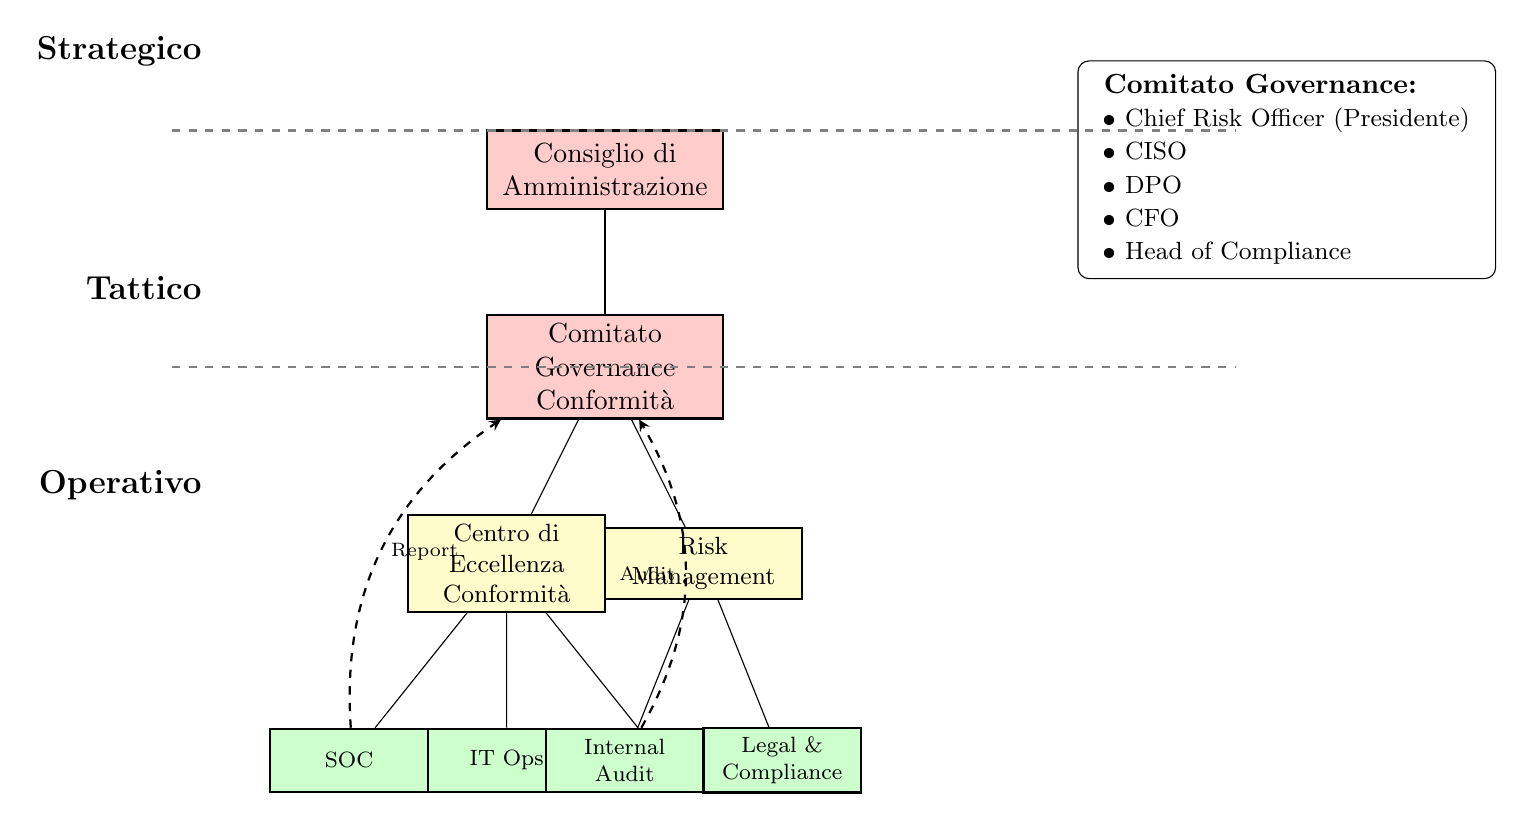
\begin{tikzpicture}[
    level 1/.style={sibling distance=4cm, level distance=2.5cm},
    level 2/.style={sibling distance=2.5cm, level distance=2.5cm},
    level 3/.style={sibling distance=2cm, level distance=2.5cm},
    exec/.style={rectangle, draw, thick, fill=red!20, minimum width=3cm, minimum height=1cm, align=center},
    tactical/.style={rectangle, draw, thick, fill=yellow!20, minimum width=2.5cm, minimum height=0.9cm, align=center, font=\small},
    operational/.style={rectangle, draw, thick, fill=green!20, minimum width=2cm, minimum height=0.8cm, align=center, font=\footnotesize},
    arrow/.style={->, >=stealth, thick}
]
    % Livello Strategico
    \node[exec] (board) {Consiglio di\\Amministrazione}
        child {node[exec] (committee) {Comitato\\Governance\\Conformità}
            child {node[tactical] (cec) {Centro di\\Eccellenza\\Conformità}
                child {node[operational] (soc) {SOC}}
                child {node[operational] (it) {IT Ops}}
                child {node[operational] (bu) {Business\\Units}}
            }
            child {node[tactical] (risk) {Risk\\Management}
                child {node[operational] (audit) {Internal\\Audit}}
                child {node[operational] (compliance) {Legal \&\\Compliance}}
            }
        };
    
    % Membri del Comitato (box laterale)
    \node[anchor=west, draw, rounded corners, fill=white] at (6,0) {
        \begin{tabular}{l}
        \textbf{Comitato Governance:} \\
        \small • Chief Risk Officer (Presidente) \\
        \small • CISO \\
        \small • DPO \\
        \small • CFO \\
        \small • Head of Compliance
        \end{tabular}
    };
    
    % Frecce di reporting
    \draw[arrow, dashed, bend left=30] (soc) to node[font=\scriptsize, right] {Report} (committee);
    \draw[arrow, dashed, bend right=30] (audit) to node[font=\scriptsize, left] {Audit} (committee);
    
    % Etichette dei livelli
    \node[anchor=east, font=\bfseries\large] at (-5,1.5) {Strategico};
    \node[anchor=east, font=\bfseries\large] at (-5,-1.5) {Tattico};
    \node[anchor=east, font=\bfseries\large] at (-5,-4) {Operativo};
    
    % Linee di separazione
    \draw[dashed, thick, gray] (-5.5,0.5) -- (8,0.5);
    \draw[dashed, thick, gray] (-5.5,-2.5) -- (8,-2.5);
\end{tikzpicture}
\caption{Modello organizzativo per la conformità integrata}
\label{fig:org_structure}
\end{figure}

% =================================================================
% FIGURA 4.5: Analisi Controfattuale - Grafico a Barre
% =================================================================
\begin{figure}[h]
\centering
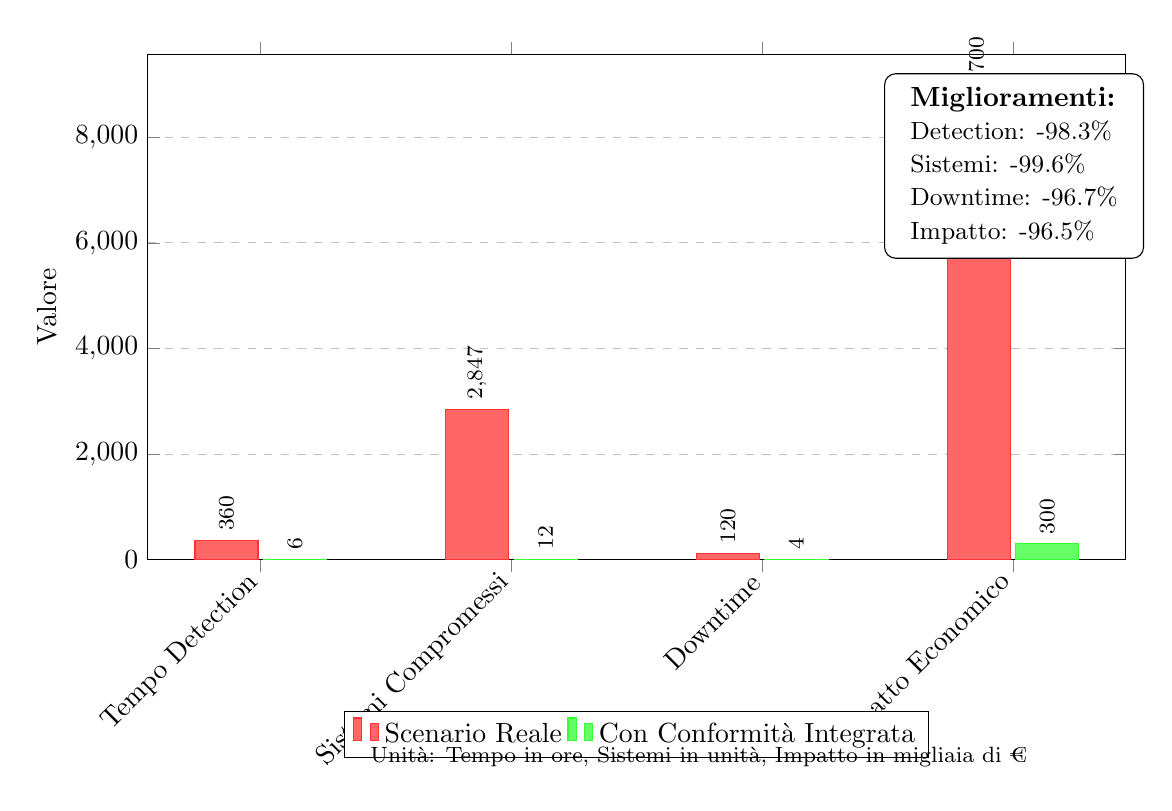
\begin{tikzpicture}
\begin{axis}[
    ybar,
    width=14cm,
    height=8cm,
    bar width=0.8cm,
    ylabel={Valore},
    symbolic x coords={Tempo Detection, Sistemi Compromessi, Downtime, Impatto Economico},
    xtick=data,
    x tick label style={rotate=45, anchor=east},
    ymin=0,
    legend style={at={(0.5,-0.3)}, anchor=north, legend columns=2},
    ymajorgrids=true,
    grid style=dashed,
    nodes near coords,
    nodes near coords style={font=\footnotesize},
    every node near coord/.append style={rotate=90, anchor=west},
    enlarge x limits=0.15,
]
    % Scenario Reale
    \addplot[fill=red!60, draw=red!80] coordinates {
        (Tempo Detection, 360)  % 15 giorni in ore
        (Sistemi Compromessi, 2847)
        (Downtime, 120)  % 5 giorni in ore
        (Impatto Economico, 8700)  % in migliaia di euro
    };
    
    % Scenario Conforme
    \addplot[fill=green!60, draw=green!80] coordinates {
        (Tempo Detection, 6)
        (Sistemi Compromessi, 12)
        (Downtime, 4)
        (Impatto Economico, 300)
    };
    
    \legend{Scenario Reale, Con Conformità Integrata}
\end{axis}

% Annotazioni con percentuali di miglioramento
\node[draw, fill=white, rounded corners] at (11,5) {
    \begin{tabular}{l}
    \textbf{Miglioramenti:} \\
    \small Detection: -98.3\% \\
    \small Sistemi: -99.6\% \\
    \small Downtime: -96.7\% \\
    \small Impatto: -96.5\%
    \end{tabular}
};

% Nota sulle unità di misura
\node[font=\footnotesize] at (7,-2.5) {
    Unità: Tempo in ore, Sistemi in unità, Impatto in migliaia di €
};
\end{tikzpicture}
\caption{Analisi controfattuale dell'impatto con conformità integrata completa}
\label{fig:controfattuale}
\end{figure}

% =================================================================
% FIGURA AGGIUNTIVA: Timeline Implementazione (Gantt Chart)
% =================================================================
\begin{figure}[h]
\centering
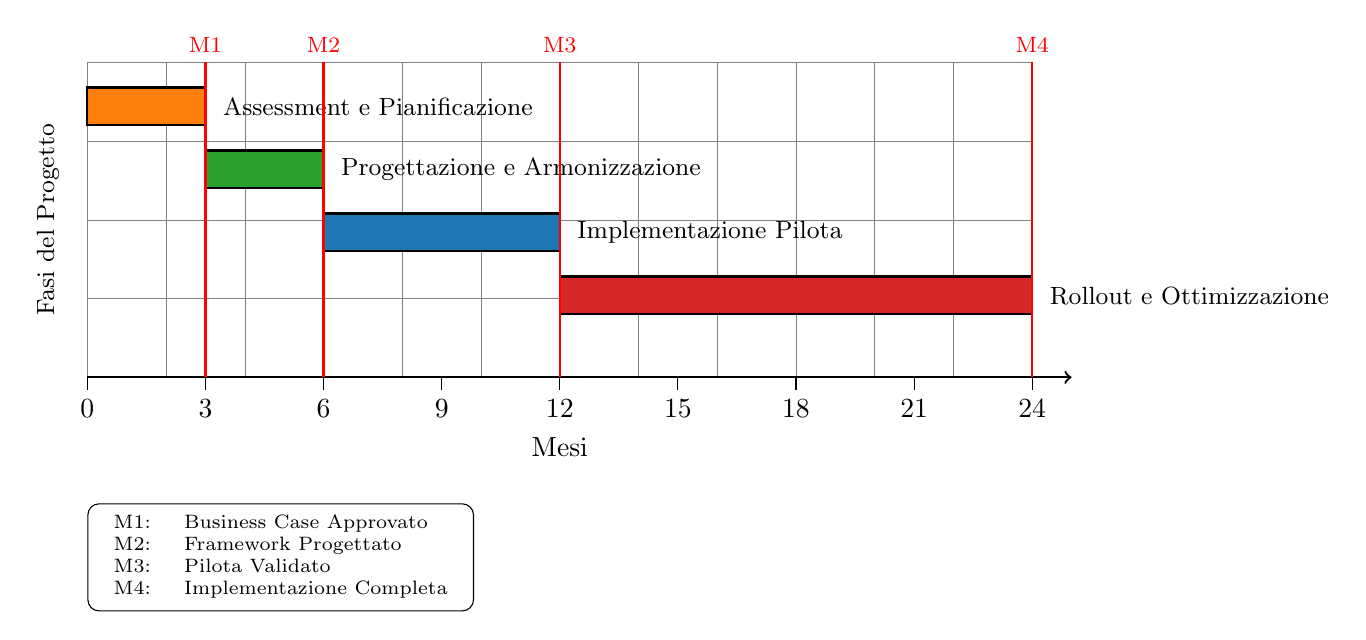
\begin{tikzpicture}[x=0.5cm, y=0.8cm]
    % Definizione colori per fasi
    \definecolor{phase1}{RGB}{255,127,14}
    \definecolor{phase2}{RGB}{44,160,44}
    \definecolor{phase3}{RGB}{31,119,180}
    \definecolor{phase4}{RGB}{214,39,40}
    
    % Griglia temporale
    \draw[gray, very thin] (0,0) grid (24,5);
    
    % Asse temporale
    \draw[thick, ->] (0,0) -- (25,0);
    \foreach \x in {0,3,6,9,12,15,18,21,24}
        \draw (\x,0) -- (\x,-0.2) node[below] {\x};
    \node[below] at (12,-0.8) {Mesi};
    
    % Fasi del progetto
    % Fase 1: Assessment
    \draw[fill=phase1, draw=black, thick] (0,4) rectangle (3,4.6);
    \node[right, font=\small] at (3.2,4.3) {Assessment e Pianificazione};
    
    % Fase 2: Progettazione
    \draw[fill=phase2, draw=black, thick] (3,3) rectangle (6,3.6);
    \node[right, font=\small] at (6.2,3.3) {Progettazione e Armonizzazione};
    
    % Fase 3: Pilota
    \draw[fill=phase3, draw=black, thick] (6,2) rectangle (12,2.6);
    \node[right, font=\small] at (12.2,2.3) {Implementazione Pilota};
    
    % Fase 4: Rollout
    \draw[fill=phase4, draw=black, thick] (12,1) rectangle (24,1.6);
    \node[right, font=\small] at (24.2,1.3) {Rollout e Ottimizzazione};
    
    % Milestone principali
    \draw[thick, red] (3,0) -- (3,5) node[above, font=\footnotesize] {M1};
    \draw[thick, red] (6,0) -- (6,5) node[above, font=\footnotesize] {M2};
    \draw[thick, red] (12,0) -- (12,5) node[above, font=\footnotesize] {M3};
    \draw[thick, red] (24,0) -- (24,5) node[above, font=\footnotesize] {M4};
    
    % Legenda milestone
    \node[anchor=north west, draw, fill=white, rounded corners, font=\scriptsize] at (0,-2) {
        \begin{tabular}{ll}
        M1: & Business Case Approvato \\
        M2: & Framework Progettato \\
        M3: & Pilota Validato \\
        M4: & Implementazione Completa
        \end{tabular}
    };
    
    % Titolo asse Y
    \node[rotate=90, font=\small] at (-1,2.5) {Fasi del Progetto};
\end{tikzpicture}
\caption{Roadmap di implementazione della conformità integrata}
\label{fig:timeline}
\end{figure}

% =================================================================
% FIGURA BONUS: Matrice di Maturità
% =================================================================
\begin{figure}[h]
\centering
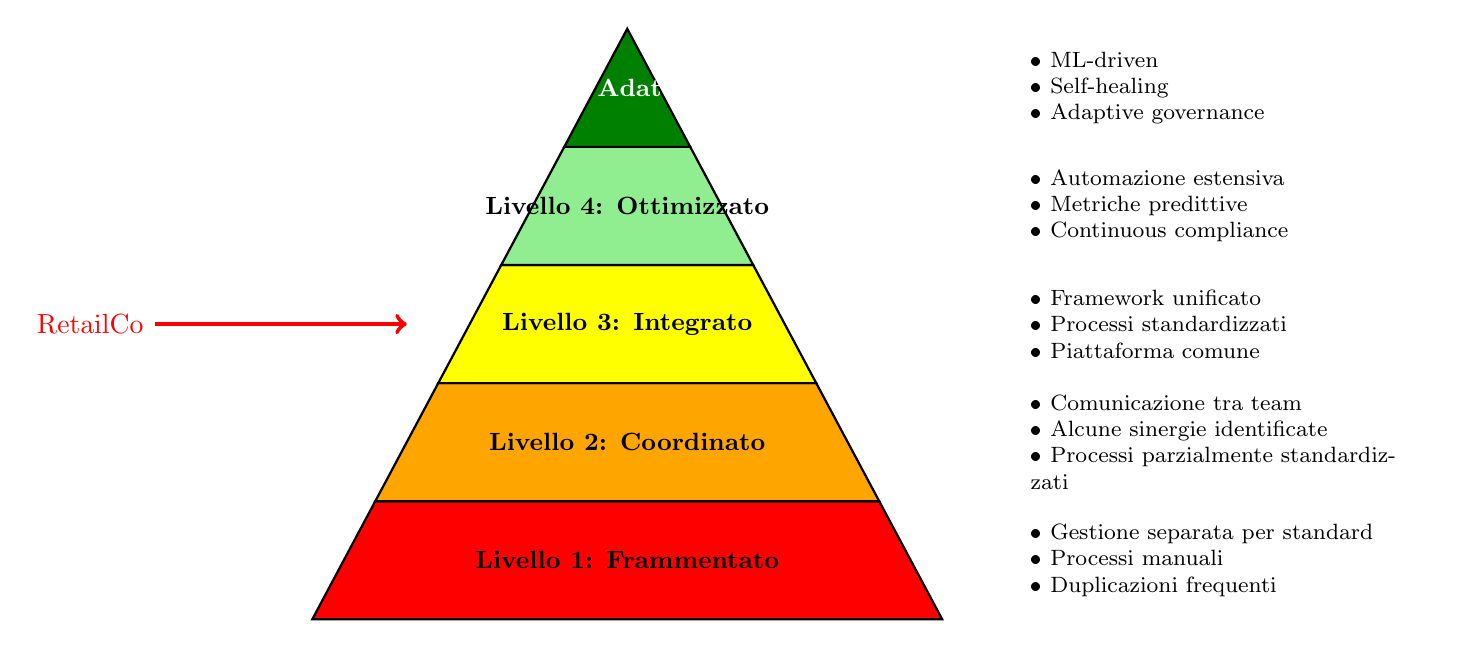
\begin{tikzpicture}
    % Definizione colori per livelli di maturità
    \definecolor{level1}{RGB}{255,0,0}
    \definecolor{level2}{RGB}{255,165,0}
    \definecolor{level3}{RGB}{255,255,0}
    \definecolor{level4}{RGB}{144,238,144}
    \definecolor{level5}{RGB}{0,128,0}
    
    % Scala di maturità (piramide)
    \coordinate (base) at (0,0);
    
    % Livello 1
    \draw[fill=level1, draw=black, thick] 
        (-4,0) -- (4,0) -- (3.2,1.5) -- (-3.2,1.5) -- cycle;
    \node[font=\small\bfseries] at (0,0.75) {Livello 1: Frammentato};
    
    % Livello 2
    \draw[fill=level2, draw=black, thick] 
        (-3.2,1.5) -- (3.2,1.5) -- (2.4,3) -- (-2.4,3) -- cycle;
    \node[font=\small\bfseries] at (0,2.25) {Livello 2: Coordinato};
    
    % Livello 3
    \draw[fill=level3, draw=black, thick] 
        (-2.4,3) -- (2.4,3) -- (1.6,4.5) -- (-1.6,4.5) -- cycle;
    \node[font=\small\bfseries] at (0,3.75) {Livello 3: Integrato};
    
    % Livello 4
    \draw[fill=level4, draw=black, thick] 
        (-1.6,4.5) -- (1.6,4.5) -- (0.8,6) -- (-0.8,6) -- cycle;
    \node[font=\small\bfseries] at (0,5.25) {Livello 4: Ottimizzato};
    
    % Livello 5
    \draw[fill=level5, draw=black, thick] 
        (-0.8,6) -- (0.8,6) -- (0,7.5) -- cycle;
    \node[font=\small\bfseries, white] at (0,6.75) {L5: Adattivo};
    
    % Descrizioni laterali
    \node[anchor=west, text width=5cm, font=\footnotesize] at (5,0.75) {
        • Gestione separata per standard\\
        • Processi manuali\\
        • Duplicazioni frequenti
    };
    
    \node[anchor=west, text width=5cm, font=\footnotesize] at (5,2.25) {
        • Comunicazione tra team\\
        • Alcune sinergie identificate\\
        • Processi parzialmente standardizzati
    };
    
    \node[anchor=west, text width=5cm, font=\footnotesize] at (5,3.75) {
        • Framework unificato\\
        • Processi standardizzati\\
        • Piattaforma comune
    };
    
    \node[anchor=west, text width=5cm, font=\footnotesize] at (5,5.25) {
        • Automazione estensiva\\
        • Metriche predittive\\
        • Continuous compliance
    };
    
    \node[anchor=west, text width=5cm, font=\footnotesize] at (5,6.75) {
        • ML-driven\\
        • Self-healing\\
        • Adaptive governance
    };
    
    % Indicatore posizione attuale (esempio)
    \draw[ultra thick, red, ->] (-6,3.75) -- (-2.8,3.75) node[left, pos=0] {RetailCo};
\end{tikzpicture}
\caption{Modello di maturità della conformità integrata (CIMM)}
\label{fig:maturity}
\end{figure}
\end{document}